\documentclass{standalone}
\usepackage{tikz}
\usetikzlibrary{arrows.meta, calc}

\begin{document}

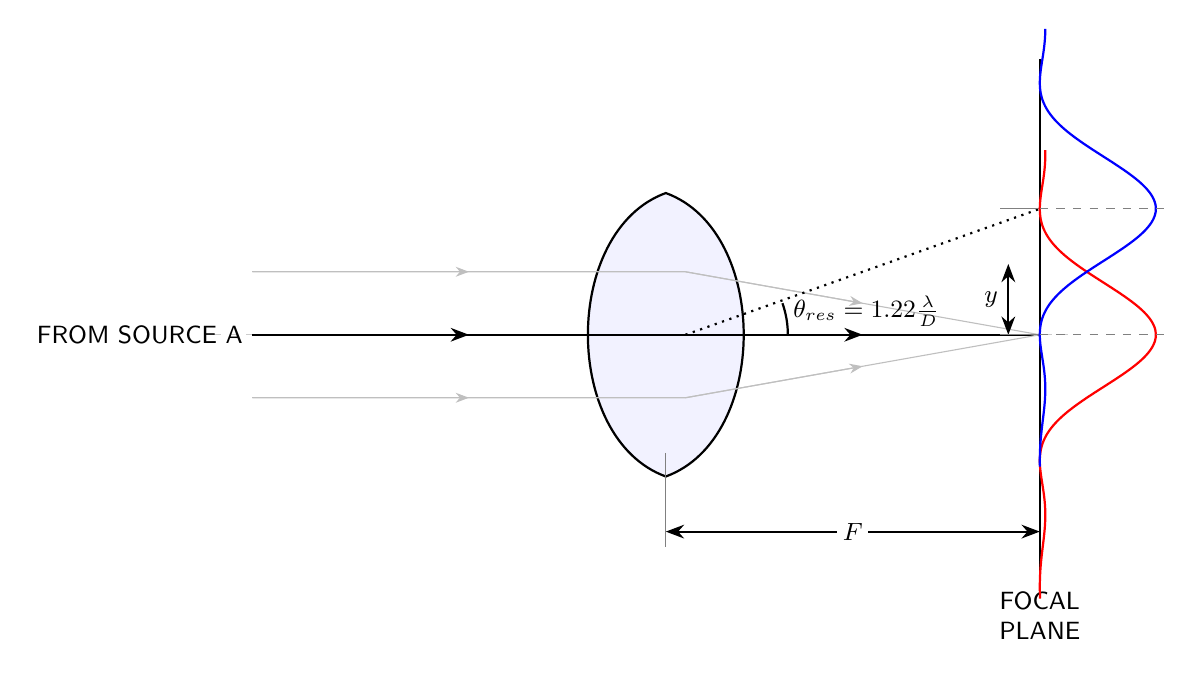
\begin{tikzpicture}[
        >=Stealth,
        font=\sffamily\small,
        ray/.style={thick, color=black},
        marginal/.style={thin, color=black!25},
        declare function={
            sinc(\x) = (\x==0 ? 1 : sin(deg(\x))/\x);
        }
    ]

    % ================= COORDINATES & PARAMETERS =================
    \coordinate (LensCenter) at (0,0);
    \def\FocalLength{4.5}
    \def\ImageOffset{1.6} % Height y of off-axis image B
    
    \coordinate (ImageA) at (\FocalLength, 0);            % Center focal point (Image A)
    \coordinate (ImageB) at (\FocalLength, \ImageOffset);   % Off-axis focal point (Image B)
    
    % Lens Parameters
    \draw[thick, fill=blue!5, draw=black] 
        (-0.25,-1.8) to[out=20, in=-20] (-0.25, 1.8) 
        to[out=-160, in=160] (-0.25,-1.8);

    % Optical Axis (Reference line)
    \draw[dashed, gray!40] (-6,0) -- (\FocalLength+0.5,0);

    % ================= SOURCE A (On-Axis Rays) =================
    \draw[marginal] (-5.5, 0.8) -- (0, 0.8) -- (ImageA);
    \draw[marginal] (-5.5, 0.8) -- (-2.75, 0.8) [arrows={-Stealth}];
    \draw[marginal] (0, 0.8) -- ($(0,0.8)!0.5!(ImageA)$) [arrows={-Stealth}];

    \draw[ray] (-5.5, 0) -- (LensCenter) -- (ImageA);
    \draw[ray] (-5.5, 0) -- (-2.75, 0) [arrows={-Stealth}];
    \draw[ray] (LensCenter) -- ($0.5*(LensCenter)+0.5*(ImageA)$) [arrows={-Stealth}];

    \draw[marginal] (-5.5, -0.8) -- (0, -0.8) -- (ImageA);
    \draw[marginal] (-5.5, -0.8) -- (-2.75, -0.8) [arrows={-Stealth}];
    \draw[marginal] (0, -0.8) -- ($(0,-0.8)!0.5!(ImageA)$) [arrows={-Stealth}];

    % Dotted line from lens center to Image B position at y
    \draw[dotted, thick, black] (LensCenter) -- (ImageB);

    % Angular arc at the lens center intersection with label \theta_{\text{res}}
    \draw [thick] (1.3,0) arc (0:19.5:1.2);
    \node at (2.3, 0.3) {$\theta_{\text{res}}=1.22\frac{\lambda}{D}$};

    % ================= LABELS & MARKS =================
    \node[left] at (-5.5, 0) {FROM SOURCE A};

    % Dimension y
    \draw[<->, thick] (\FocalLength-0.4, 0) -- (\FocalLength-0.4, 0.9) 
        node[midway, left] {$y$};
    \draw[thin, gray] (ImageA) -- (\FocalLength-0.5, 0);
    \draw[thin, gray] (ImageB) -- (\FocalLength-0.5, \ImageOffset);

    % Dimension F
    \draw[<->, thick] (-0.25, -2.5) -- (\FocalLength, -2.5) 
        node[midway, fill=white, inner sep=2pt] {$F$};
    \draw[thin, gray] (-0.25, -1.5) -- (-0.25, -2.7);
    \draw[thin, gray] (\FocalLength, -0.2) -- (\FocalLength, -2.7);

    % ================= FOCAL PLANE & ROTATED DIFFRACTION PLOT =================
    % Focal Plane Line
    \draw[thick] (\FocalLength, -3.0) -- (\FocalLength, 3.5);
    \node[below=4pt, align=center] at (\FocalLength, -3.0) {FOCAL\\PLANE};

    % Scope shifted to Image A baseline and rotated -90 degrees
    \begin{scope}[shift={(\FocalLength, 0)}, rotate=-90, scale=0.67]
        \def\xR{0.0}            % Red peak aligned with Source A (y=0)
        \def\xB{-2.388}         % Blue peak aligned with Source B (y=1.6 scaled: -1.6 / 0.67 = -2.388)
        \def\dx{2.388}          % Spacing matching image separation

        % Red diffraction pattern
        \draw[red, thick, domain=-3.5:5.0, samples=300, smooth] 
            plot (\x, {2.2 * pow(sinc(3.14159 * (\x - \xR) / \dx), 2)});

        % Blue diffraction pattern
        \draw[blue, thick, domain=-5.8:2.5, samples=300, smooth] 
            plot (\x, {2.2 * pow(sinc(3.14159 * (\x - \xB) / \dx), 2)});

        % Dashed alignment lines for the two central maxima
        \draw[dashed, gray] (\xR, 0) -- (\xR, 2.5);
        \draw[dashed, gray] (\xB, 0) -- (\xB, 2.5);

        % Arrow connecting the two central maxima
    \end{scope}

\end{tikzpicture}

\end{document}